% Paperformat
\documentclass[a4paper, 12pt]{scrartcl}
\usepackage{cite}
\usepackage{ragged2e}
\usepackage{url}
\usepackage{bm} % bold math
\usepackage{nccmath} % medium fraction with mfrac 
\usepackage{amssymb}
\usepackage{graphicx}
\usepackage{amsthm} % theorems
\usepackage{hyperref}
\usepackage{float}

\newtheorem{theorem}{Theorem}[section]
\begin{document}

\begin{titlepage}
	\vspace*{\stretch{1}}
	\begin{center}
		{\Large\bfseries Bachelor Thesis}           \\[6.5ex]
		
		{\huge\bfseries Visualizing Dynamic Programming on Tree Decompositions}                  \\[6.5ex]
		
		\vspace{6ex}
				
		\textsc{\Large Martin Röbke}    \\[3ex]
		{\Large born: 04.03.1995 in Dresden, Germany}    \\[2ex]
		{\Large matriculation number: 3949819}    \\[2ex]
		{\Large martin.roebke@tu-dresden.de}    \\[2ex]
		\textsc{\large 
			}             \\[12ex]
		\vfill
		{\Large Technische Universität Dresden}               \\
		Faculty of Computer Science \\
		International Center For Computational Logic 		\\[5ex]
		
		{\Large Supervisor: Dr. Johannes Fichte}\\[2ex]
		{\Large Second evaluator:  Prof. Dr. rer. nat. Stefan Gumhold}\\[5ex]
		
		\vfill
		Dresden, \today
	\end{center}
	\vspace{\stretch{2}}
\end{titlepage}


%==============================================================================
%============== ABSTRACT ======================================================
%==============================================================================
\section*{Abstract}
\vspace{4ex}
The thesis is about a practical and lightweight implementation for visualizing dynamic programming on tree decompositions.
I created the python-package\href{https://pypi.org/project/tdvisu}{tdvisu} for the purpose of visualizing, teaching and analyzing the solving process of MSOL-problems using tree decomposition. \\
Intended audience: 
\begin{itemize}
	\item  Developer of dynamic programming on tree decompositions for debugging.
	\item Researcher of such algorithms for comparisons and visualizations.
	\item Teachers or students wanting some automatic visualization of their examples and the dynamic-solving-process.
\end{itemize} 

As two reference implementations of dynamic programming on tree decompositions we chose the projects \href{https://github.com/daajoe/GPUSAT}{GPUSAT} and \href{https://github.com/hmarkus/dp_on_dbs}{dpdb}.

\newpage

%  table
\tableofcontents

% chapter on next page
\newpage

%==============================================================================
%============== INTRODUCTION ==================================================
%==============================================================================

\section{Introduction}
Graphs are increasingly interesting in scientific work.
The idea for this project comes from my supervisor Dr. Johannes Fichte, who works on and with many projects such as the ones listed above on solving monadic second order logic (MSOL\cite{Courcelle2012}) problems using highly parallelized architectures like graphics processing units or state of the art databases.
One early implementation is published in \cite{evaluationMSO} where for different real world examples the results looked promising
These projects are very competitive ????REF????? for solving even large instances of those problems.

intro. mit motivation und related work, state of the art, advancements.


Visualization Pipeline

Stand Umsetzung, Tools: Slack, Trello, GitHub, Presentations

%==============================================================================
%============== BACKGROUND ====================================================
%==============================================================================

\newpage
\section{Background}
\textit{This chapter provides the reader with a brief background for this work}.

We begin with a description on SAT and \#SAT as examples for a very general problem that can be described with monadic second order logic (MSOL).
Furthermore the general case of MSOL will be described, as well as the \textit{DIMACS}-file-format used in the projects.
The following section describes Tree Decompositions (TDs) which are the basis for our visualization. 
Finally we shortly discuss Courcelle's Theorem~\cite{Courcelle2012} as a related method of solving these problems.

\subsection{Boolean satisfiability problem}
\url{https://en.wikipedia.org/wiki/Boolean_satisfiability_problem}

SAT was the first known NP-complete problem, shown by Stephen Cook at the University of Toronto in 1971 \cite{SAT1971}

\begin{align*}
\text{literal}&\equiv \text{boolean variable v or its negation} \\
\text{clause}&\equiv \text{finite set of literals, interpreted as the disjunction} \\
\text{unit}&\equiv \text{clause with $|$c$|$=1} \\
\text{CNF formula}&\equiv \text{set of clauses, interpreted as their conjunction} \\
\text{var}&\equiv \text{set of variables contained in the clause or clause set C} \\
\text{assignment}&\equiv \text{$\alpha $:var(C) $\to $ \{0,1\}} \\
\text{satisfiedclause}&\equiv \text{if $\exists $v $\in $ var(c), v$\in $c and $\alpha $(v)=1 or $\neg $v$\in $c and $\alpha $(v)= 0. Otherwise falsified}\\ 
\text{satisfiedform}&\equiv \text{each clause in the formula is satisfied by assignment} \\
\end{align*}

Connection to graphs with \cite{DiplomarbeitZisser}

SAT Handbook:
Even finding a single solution can be a challenge
for such problems; counting the number of solutions is much harder.Not
surprisingly, the largest formulas we can solve for the model counting problem
with state - of - the - art model counters are orders of magnitude smaller than the
formulas we can solve with the best SAT solvers. Generally speaking, current
exact counting methods can tackle problems with a couple of hundred variables, while approximate counting methods push this to around 1, 000 variables.


\subsection{Monadic Second Order Logic}
See also figure~\ref{fig:logictheory}.

Explain graphs?Node, Edge

MSO graph properties are "fixed-parameter-tractable" with respect to clique-width and tree-width. 
\url{https://www.youtube.com/watch?v=hZI-wANHO1w} 5th workshop on Graph Classes, Optimization, and Width Parameters (GROW 2011)
2011-10-28.
MSO counting (k-colorings )and optimizing (distance between two vertices...) functions.
Interested in MSO logic over graphs.

Two types of MSO formulas \textit{or logical graph representations}.
\begin{itemize}
	\item MSO formulas
	\item MSO$_{2}$ formulas with edge quantification $\equiv$ MSO formulas over incidence graphs
\end{itemize}
\begin{itemize}
	\item G=(vertices, edges as binary relation)
	\item INC(G) = (vertices and edges, Inc)
		for G undirected: Inc(e,v) <-> v is a vertex of edge e
\end{itemize}
\begin{itemize}
	\item FPT for clique width
	\item FPT for tree-width
\end{itemize}
This can also be done for directed graphs!

Typical MSO$_{2}$ graph properties:

has a perfect matching
has a Hamiltonian circuit
spanning tree of degree $\le$ 3

The expressions have the form: "There exists a \textbf{set of edges} that is..." can not be transferred into "set of vertices"

\url{https://youtu.be/Wyn3djrYg7c?t=1385} Bruno Courcelle: Recognizable sets of graphs: algebraic and logical aspects 
\url{https://library.cirm-math.fr/Record.htm?idlist=2&record=19276851124910940339}
Recording during the thematic meeting: "Frontiers of reconnaissability" the April 29, 2014 at the Centre International de Rencontres Mathématiques (Marseille, France)

FPT for model checking:
An algorithm is FPT if it takes time $f(k)\cdot n^{c}$ for some fixed function f and constant c. The size of the input is n. 
The value k is a parameter of the input. 
This algorithm is then usable for small values of k. usually tree-width and clique width.


\subsection{DIMACS Format}
Developed in 1993 at Rutgers University.
DIMACS (the Center for Discrete Mathematics and Theoretical Computer Science)

Wolfram Language fully supports the DIMACS format for storing a single undirected graph.
\url{https://reference.wolfram.com/language/ref/format/DIMACS.html}

DIMACS CNF: This format is used to define a Boolean expression, written in conjunctive normal form.
\url{https://people.sc.fsu.edu/~jburkardt/data/cnf/cnf.html}

Other formats for WMC, different graphs...

Supported also in Maple \url{https://www.maplesoft.com/support/help/maple/view.aspx?path=Formats/CNF}

Examples in appendix

\subsection{Tree Decomposition}
\cite{DiplomarbeitZisser}chapter 2.2
Tree decompositions were originally introduced by Robertson and Seymour \cite{ROBERTSON198449} in 1984.
A \textit{tree decomposition} (TD) of a graph G is a pair $(T, \chi)$. $T$ is a tree and $\chi$ is a mapping which assigns each node $n~\in~V(T)$ 
a set $\chi(n) \subseteq V(G)$ called a \textit{bag}. Then $(T, \chi)$. $T$ is a TD if the following conditions hold:

\begin{itemize}
	\item[1.] for each vertex $v(n) \in V(G)$ there is a node $n \in V(T)$ such that $v \in \chi(n)$
	\item[2.] for each edge $(x,y) \in E(G)$ there is a node $n\in V(T)$ such that $x,y \in\chi(n)$
	\item[3.] if $x,y,z \in V(T)$ and $y$ lies on the path from x to z then $\chi(x) \cap \chi(z) \subseteq \chi(y)$.
\end{itemize}
The width $width(T)$ of a tree decomposition $T$ is $max_{n\in V(T)}(|\chi(n)|)-1$.
The tree width of a graph is the \textit{minimal width} over all tree decompositions of the graph.

!!!Example (can take one from the visualizations) also in \cite{pcgp2019} page 169
\subsection{Courcelle's Theorem}
\begin{quotation}
	Every graph property definable in monadic second-order logic (MSO) is decidable in linear time on graphs of bounded tree-width.\\
	{\small Courcelle, Bruno (1990)}\footnote{Courcelle, Bruno "The monadic second-order logic of graphs. I. Recognizable sets of finite graphs",\\ Information and Computation, 85 (1990) no. 1: 12-75}
\end{quotation}

For all $k \in \mathbb{N}$ and MSO-sentences F is the decision problem for a given graph G, whether $G \models F$ is true, in time $2^{p(tw(G))} \cdot |G|$ with a polynom p decidable.
\begin{itemize}
	
	\item \emph{drawback:} still expensive ($2^{p(tw G)}$, $2^{2^{(\#Q)}}$, large constants) \smallskip 

\end{itemize}

The workflow then looks like we see in figure~\ref{fig:UsageCourcelle}.

\begin{figure}[H]
	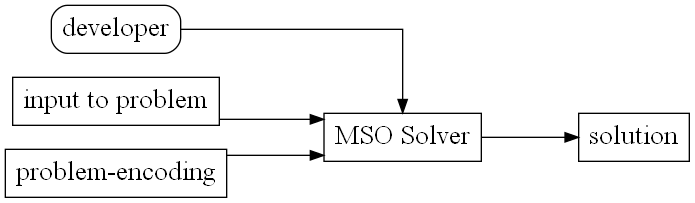
\includegraphics[height=0.2\textheight]{images/UsageCourcelle.gv.png}
	\caption{Implementation of the theorem}
	\label{fig:UsageCourcelle}
\end{figure}
%==============================================================================
%============== CONCEPT =======================================================
%==============================================================================
\newpage
\section{Concept}
What I do and why I did it
Steps in Trello, Issues, Commits
Research: language (python - explain) graph-construction (graphviz vs networkX), examples (diploma at first). 

%==============================================================================
%============== PROJECT =======================================================
%==============================================================================
\newpage
\section{My Visualization Project}

Pip, requirements files, virtual environments and how to pick quality Python libraries:
\url{https://realpython.com/products/managing-python-dependencies/?utm_source=drip&utm_medium=email&utm_campaign=productfooter&utm_content=mpd}


The first stages were in \url{https://github.com/VaeterchenFrost/gpusat-VISU} and the first releases of the source code outsourced to\url{https://github.com/VaeterchenFrost/tdvisu}

The objective of this project was/is to support the visualization mainly to document and improve the development efforts of dynamic programming on tree decompositions.

The tree decompositions in every tested application were provided by the utility \url{https://github.com/mabseher/htd} (small but efficient C++ library for computing (customized) tree and hypertree decompositions).
Files / Classes / Methods
Current 
perspective 
Checking with www.deepcode.ai

\newpage
\subsection{Integration in GPUSAT}
Windows opencl driver problem: ERROR: clBuildProgram(-9999)

Programm \url{https://github.com/VaeterchenFrost/GPUSAT} \\
Differences: \url{https://github.com/daajoe/GPUSAT/compare/master...VaeterchenFrost:master}  Commits 142 Files changed 94 
Nagoya talk:
Graphs for performance are Ordered by used time per algorithm - gpusat quite good

Working with cmake remotly. ssh @(sg1.)dbai.tuwien.ac.at
CPU branch wasn't working.
Only AMD/Nvidia graphics  with respective flags.

First steps:
Connect ssh
mkdir Ba
cd Ba
git clone https://github.com/mabseher/htd.git
 cd htd/
 cmake .
 make -B -j1 
 make test
 (100pct tests passed, 0 tests failed out of 38                                                                                                                                                                                                                                                                                                             Total Test time (real) =   0.81 sec )\\

git clone https://github.com/VaeterchenFrost/GPUSAT.git
Adding include\_directories (/home/roemar/Ba/htd/
include) to CMakeLists.txt \\
find\_library(HTD\_LIB htd /home/roemar/Ba/htd/lib)
find\_library(HTD\_IO\_LIB htd\_io /home/roemar/Ba/htd/lib) 
cmake - L~/Ba/GPUSAT/build
-- Configuring done
-- Generating done
-- Build files have been written to : /home/roemar/Ba/GPUSAT/build-- Cache values 
\\
Common commands
cd Ba/GPUSAT      
date \&\& make \&\& scp ./gpusat mroebke@128.131.196.128:~/Ba/GPUSAT/GPUSAT/build/december

The CUDA Remote had no cmake so I built the projects on the Proxy tuwien.

\subsubsection{Class Graphoutput}
First steps in automatically visualizing the solving process with its tree decomposition.
Outputs a .dot graph !!!EXAMPLE!!! with the bags and their solution nodes.

Additionally two functions to generate a Neo4J Cypher ***Link*** Query with:
\begin{itemize}
	\item one graph representing the SAT formula and  queries to construct incidence, dual and primal representations.
	output as satFile = "cypherSatFormula.txt"
	\item a graph representing the tree decomposition of the primal graph with it's bags containing variables.
	output as tdFile = "cypherTreedec.txt"
\end{itemize}
\subsubsection{Class SolverVisualization}

Umsetzung Special fork connecting the Visualization directly to the 
Beispiel
\newpage
\subsection{Integration in dpdb}
Programm
Umsetzung
Beispiel

%==============================================================================
%============== APPLICATION ===================================================
%==============================================================================
\newpage
\section{Application and Images }

%==============================================================================
%============== SUMMARY =======================================================
%==============================================================================
\newpage
\section{Summary and Outline}
What is achieved?
What worked good, what bad?
\bibliography{bibtex}{}
\bibliographystyle{ieeetr}

%==============================================================================
%============== APPENDIX ======================================================
%==============================================================================
\newpage
\appendix
\section{Images}
\begin{figure}[H]
	\centering
	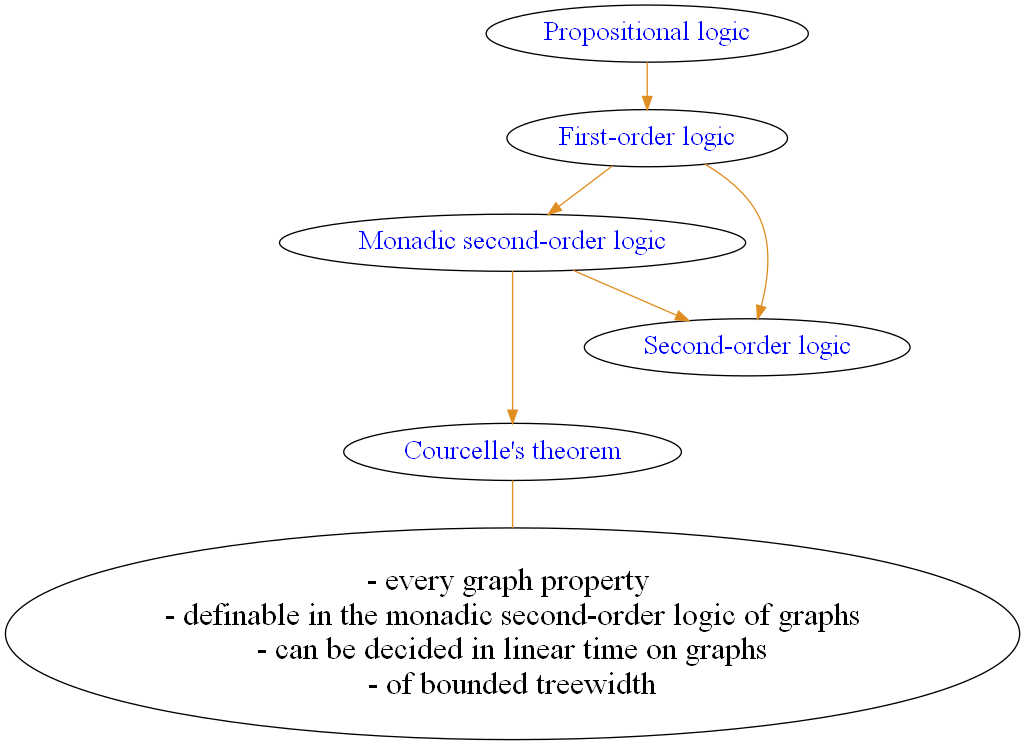
\includegraphics[width=0.8\linewidth]{images/logictheory.png}
	\caption{From propositional logic to monadic second order logic and Courcelle's Theorem}
	\label{fig:logictheory}
\end{figure}
\end{document}